%\clearpage

\appendix
\renewcommand{\appendixname}{Anexos}
\renewcommand{\appendixtocname}{Anexos}
\renewcommand{\appendixpagename}{Anexos}
\clearpage
\addappheadtotoc
%\appendixpage %Agrega una pagina en blanco q en el medio Dice Anexo en grande..



    \begin{minipage}{0.95\textwidth}
    \chapter{Diagrama del modelo de casos de uso}
    %\section{Diagrama del modelo de casos de uso}
    	\leftline{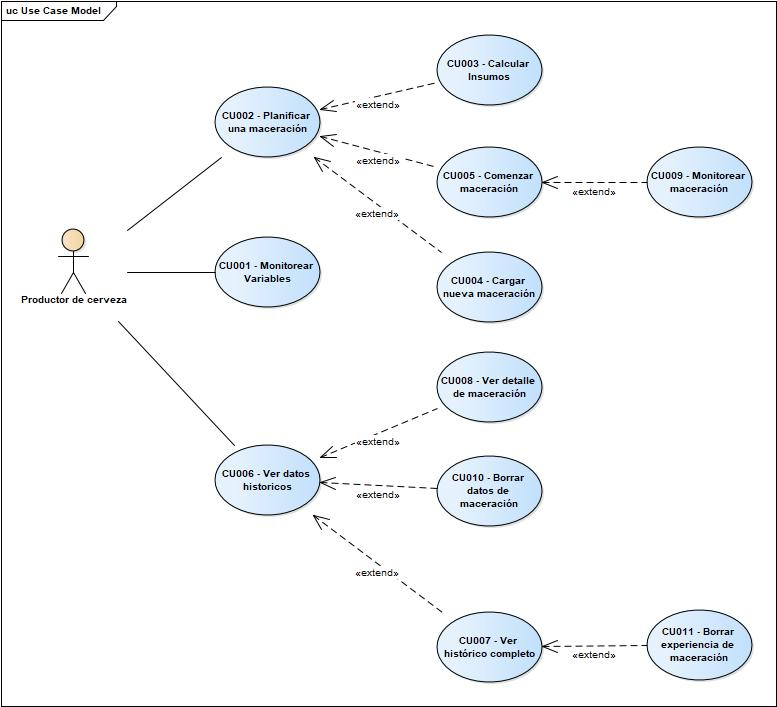
\includegraphics[scale=0.55]{ModelodeCasosdeUso.jpg}}
    	\captionof{figure}{Diagrama de Casos de Uso}
	    \label{DiagCU}
	\end{minipage}


    \begin{minipage}{0.95\textwidth}
    \chapter{Diagrama de base de datos del componente de Hardware}
        \centering
        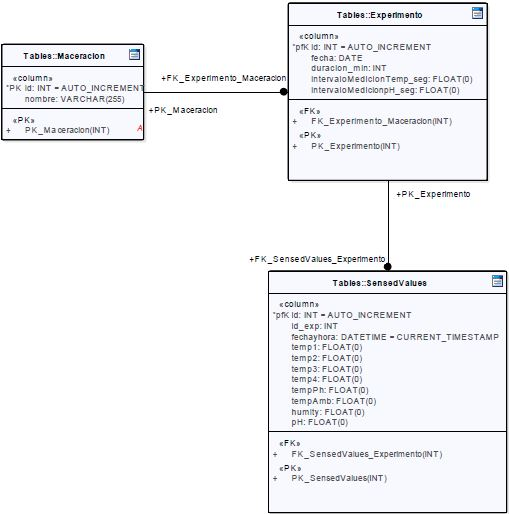
\includegraphics[scale=1]{diagramaBD-Rasp.jpg}
        \captionof{figure}{Diagrama de diseño de Base de Datos}
        \label{fig:DiagramaBdRasp}
    
    \end{minipage}
    
    \begin{minipage}{0.95\textwidth}
    \chapter{Esquema de conexión de la estación de recolección de datos}
        \centering
        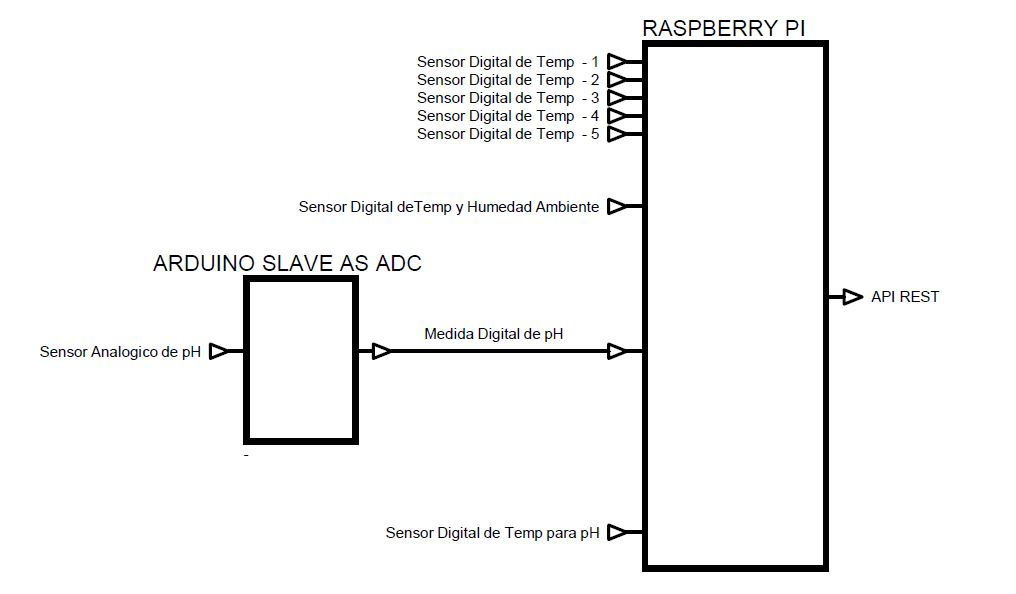
\includegraphics[scale=0.55]{EsquemaHardware.jpg}
        \captionof{figure}{Esquema simplificado de las conexiones}
        \label{fig:EsquemaHardware}
    \end{minipage}
    
%---------------------- MOCK UP ----------------------------------------
    \begin{minipage}{0.95\textwidth}
    \chapter{Diseño de Interfaz de Usuario}
    %\section{Diseño de Interfaz de Usuario}
        \centering
        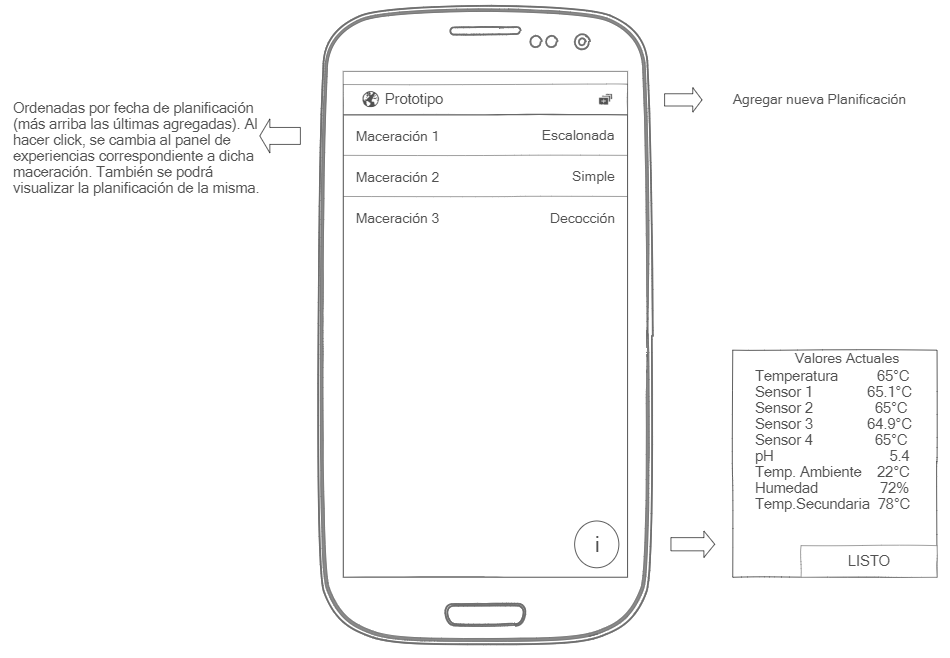
\includegraphics[scale=0.55]{Anexo/MockUp/MainActivity.jpg}
        \captionof{figure}{Pantalla Principal}
        \label{fig:MockUpMainActivity}
    \end{minipage}
    
    \begin{minipage}{0.95\textwidth}

        \centering
        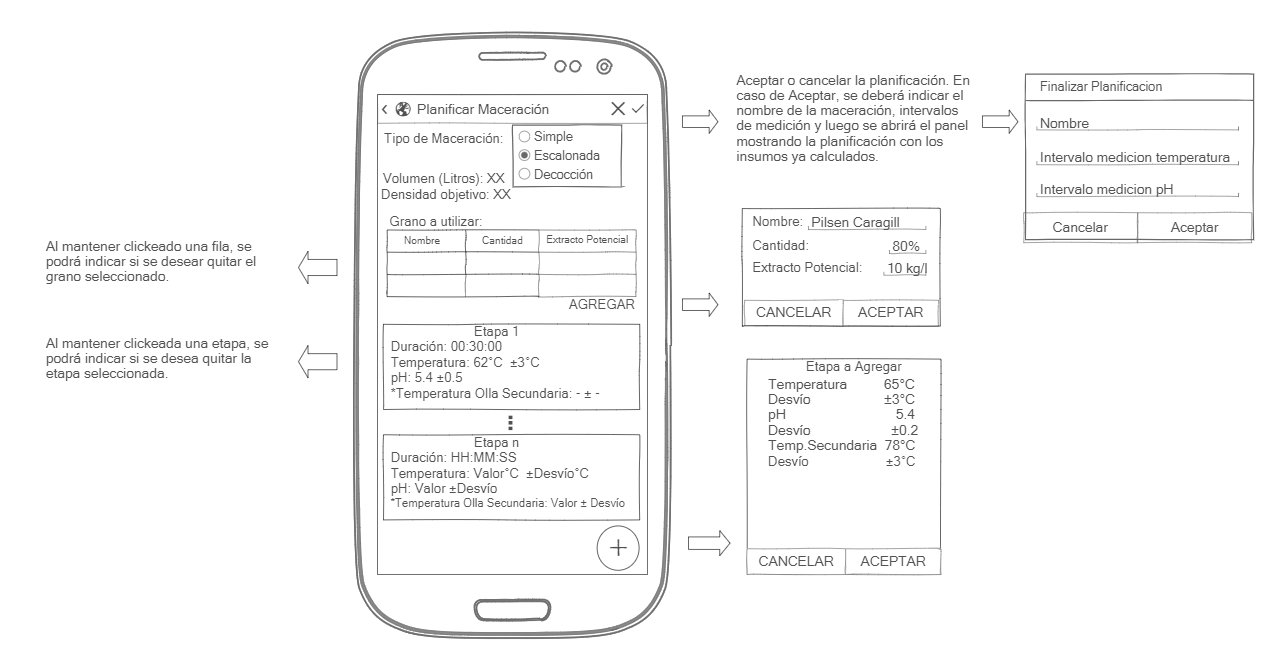
\includegraphics[scale=0.55, angle =90]{Anexo/MockUp/PlanningActivity.jpg}
        \captionof{figure}{Pantalla de planificación de maceración}
        \label{fig:MockUpPlanningActivity}
    \end{minipage}
    
    \begin{minipage}{0.95\textwidth}

        \centering
        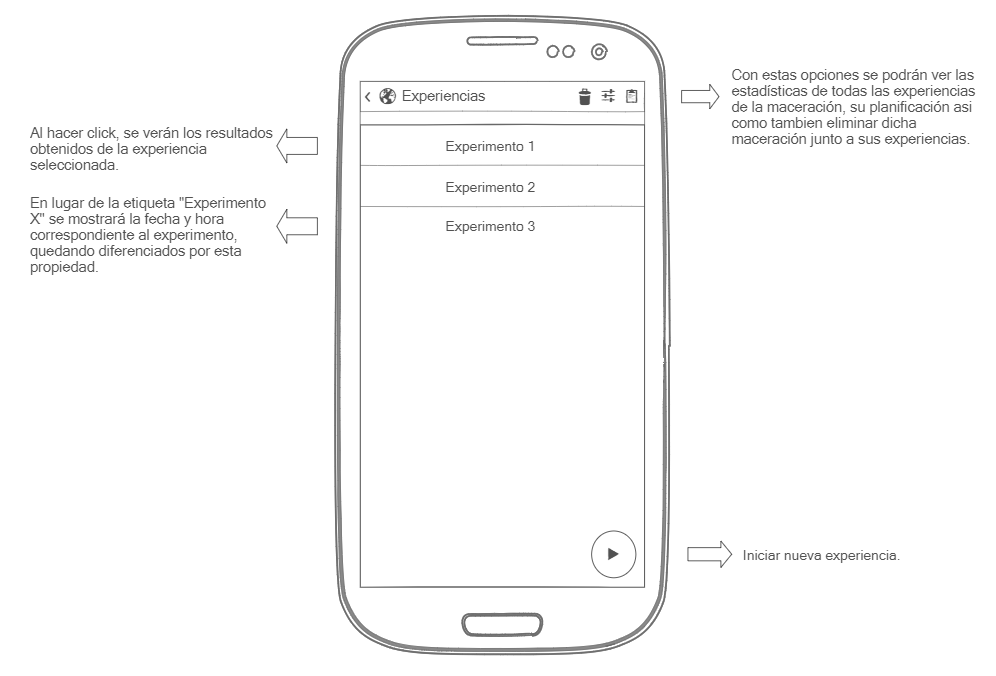
\includegraphics[scale=0.55]{Anexo/MockUp/ExperimentActivity.jpg}
        \captionof{figure}{Pantalla con lista de experimentos de una maceración}
        \label{fig:MockUpExperimentActivity}
    \end{minipage}
    
    \begin{minipage}{0.95\textwidth}

        \centering
        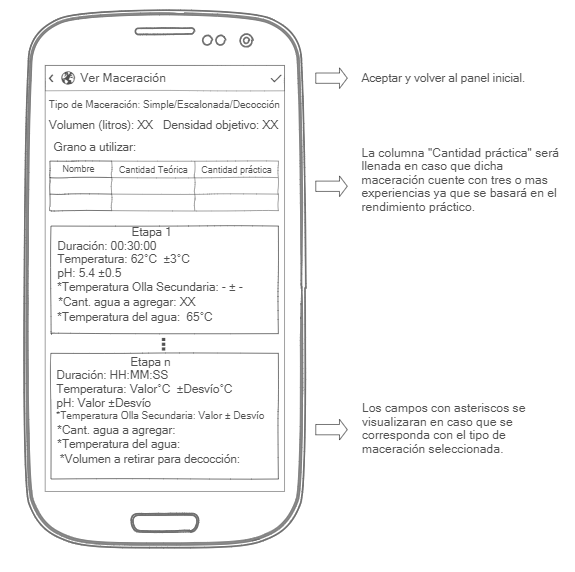
\includegraphics[scale=0.7]{Anexo/MockUp/InfoMash.jpg}
        \captionof{figure}{Pantalla con información de la maceración}
        \label{fig:MockUpInfoMash}
    \end{minipage}
    
    \begin{minipage}{0.95\textwidth}

        \centering
        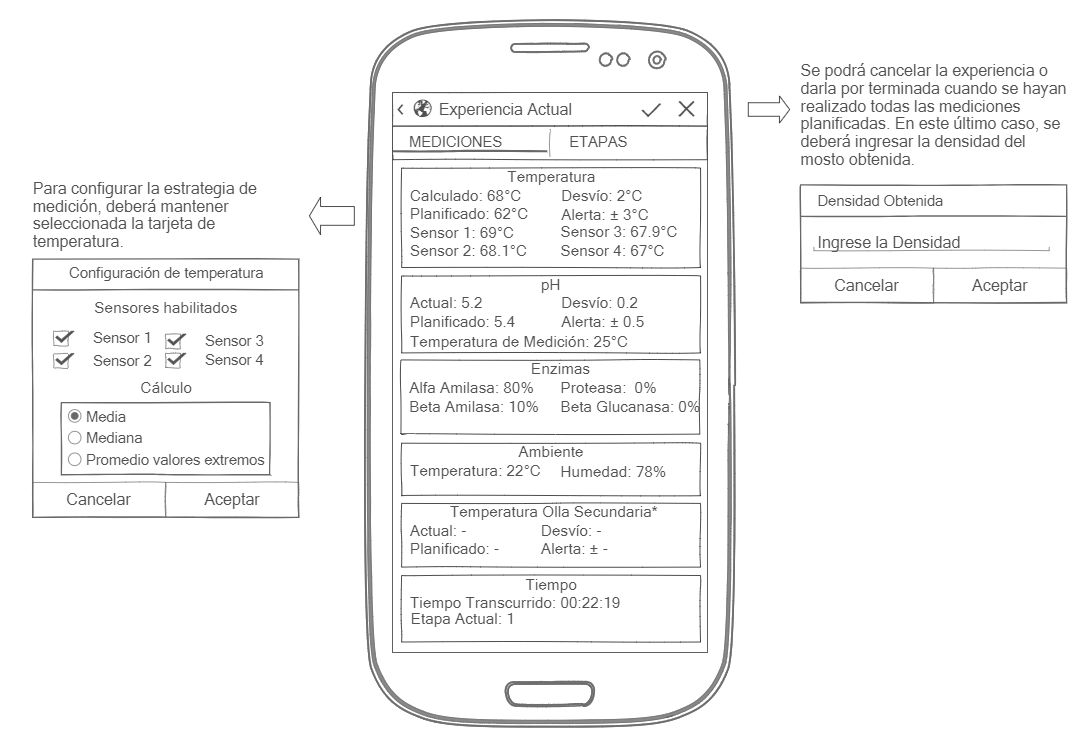
\includegraphics[scale=0.5]{Anexo/MockUp/CurrentExperience-MeasureFragment.jpg}
        \captionof{figure}{Pantalla de mediciones del experimento en ejecución}
        \label{fig:MockUpCurrentExperienceFragment}
    \end{minipage}
    
    \begin{minipage}{0.95\textwidth}

        \centering
        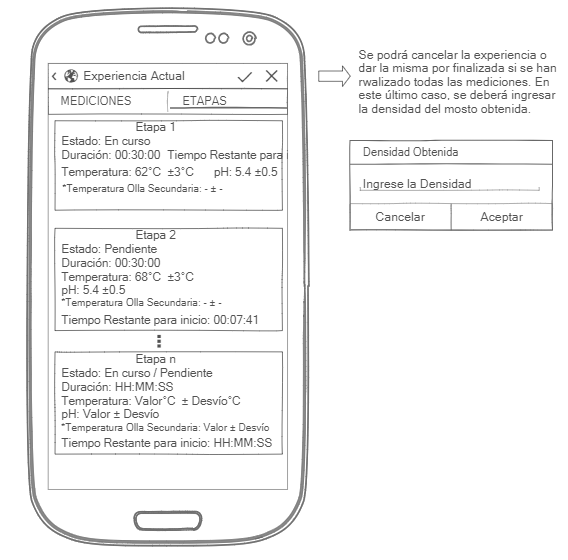
\includegraphics[scale=0.7]{Anexo/MockUp/CurrentExperience-StageFragment.jpg}
        \captionof{figure}{Pantalla con información de las etapas del experimento en ejecución}
        \label{fig:MockUpStageFragment}
    \end{minipage}
    
    \begin{minipage}{0.95\textwidth}

        \centering
        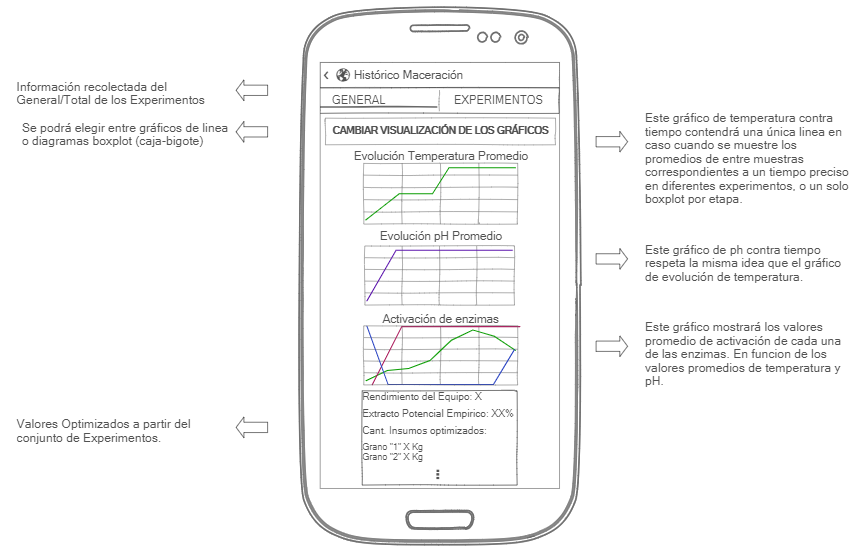
\includegraphics[scale=0.7]{Anexo/MockUp/MashExpHistoryActivity-GeneralFragment.jpg}
        \captionof{figure}{Pantalla con información estadística descriptiva de mediciones y de optimización de insumos y rendimiento}
        \label{fig:MockUpGeneralFragment}
    \end{minipage}
    
    \begin{minipage}{0.95\textwidth}

        \centering
        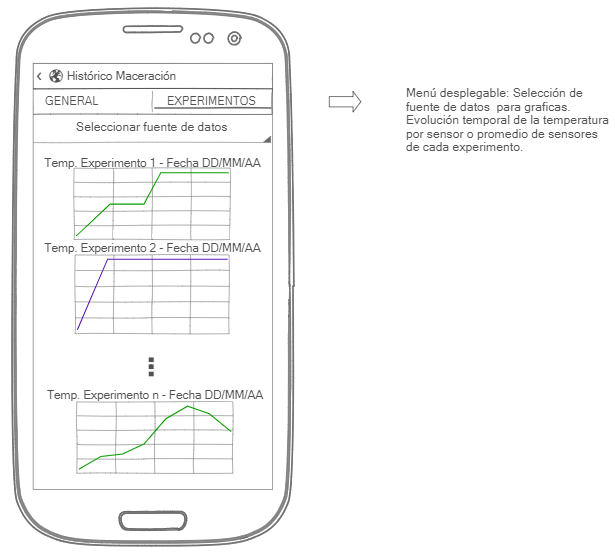
\includegraphics[scale=0.7]{Anexo/MockUp/MashExpHistoryActivity-ExperimentFragment.jpg}
        \captionof{figure}{Pantalla con información estadística descriptiva de mediciones de temperatura de cada experimento}
        \label{fig:MockUpExperimentFragment}
    \end{minipage}
    
   \begin{minipage}{0.95\textwidth}

        \centering
        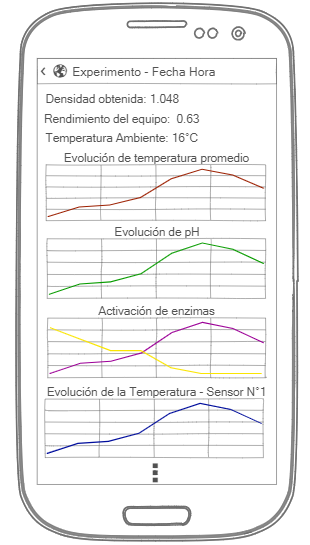
\includegraphics[scale=0.7]{Anexo/MockUp/DetailExperimentActivity.jpg}
        \captionof{figure}{Pantalla con información detalladas de los resultados de cada experimento}
        \label{fig:MockUpDetailExperimentActivity}
    \end{minipage}
    
%-------------------------- DIAGRAMAS DE CLASE --------------------------- 
    \begin{minipage}{0.95\textwidth}
    \chapter{Diagramas de clases}
    %\begin{figure}
        \centering
        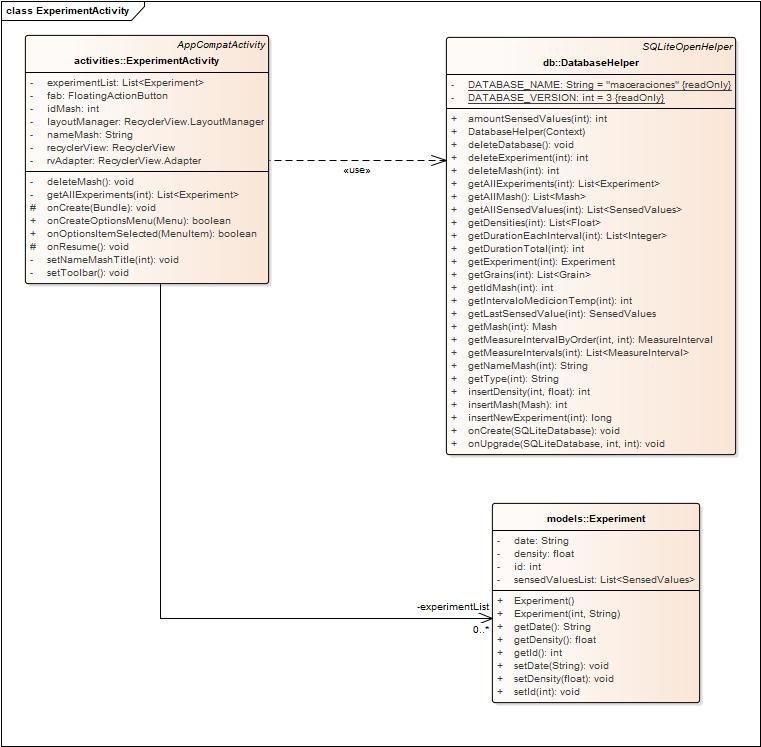
\includegraphics[scale=0.55, angle=90]{Anexo/DiagramasClase/ExperimentActivity.jpg}
        \captionof{figure}{Diagrama de clases de ExperimentActivity}
        \label{fig:DiagClaseExperimentActivity}
    %\end{figure}
    \end{minipage}
    
    %\begin{minipage}{0.95\textwidth}
            \begin{figure}
                \centering
                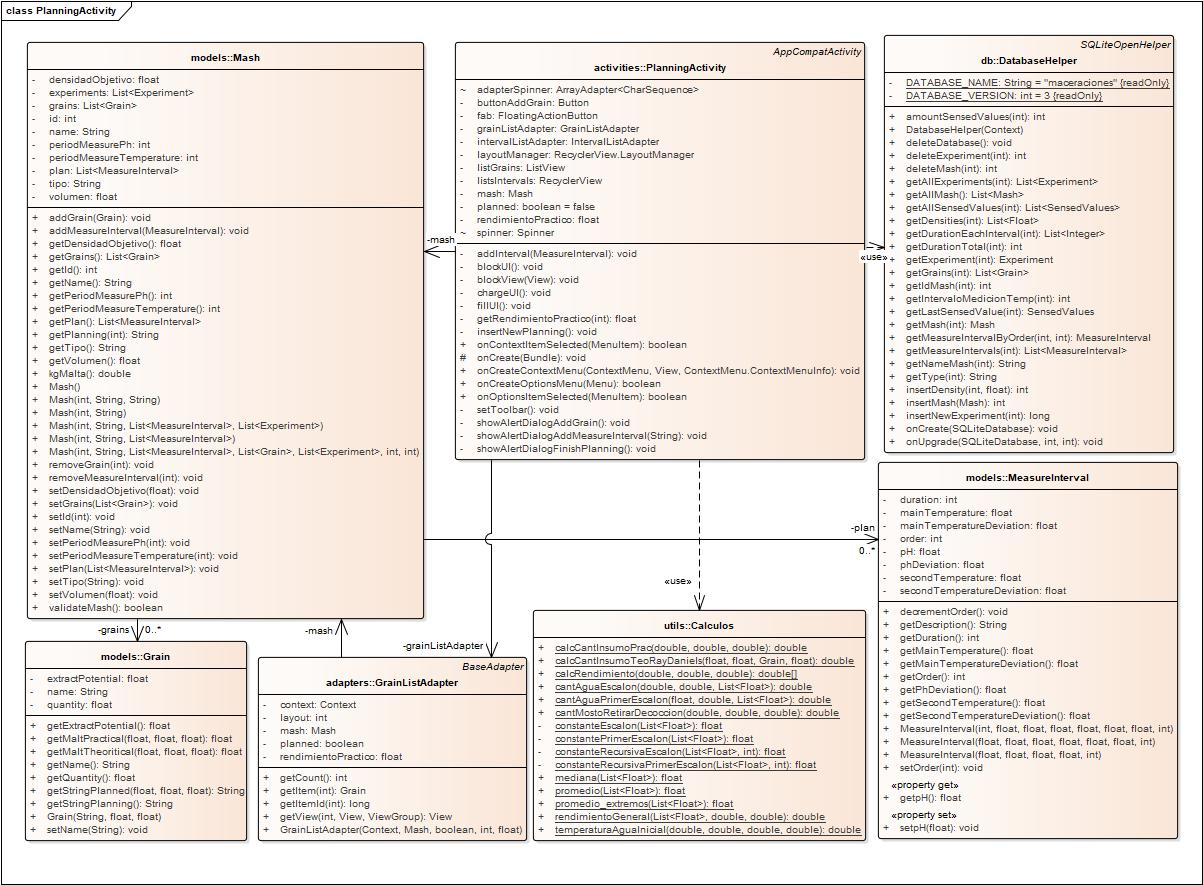
\includegraphics[scale=0.5, angle=90]{Anexo/DiagramasClase/PlanningActivity.jpg}
                \captionof{figure}{Diagrama de clases de PlanningActivity}
                \label{fig:DiagClasePlanningActivity}
            \end{figure}
    %\end{minipage}
    
    
    \begin{figure}
        %\section{Diagramas de clases}
        \centering
        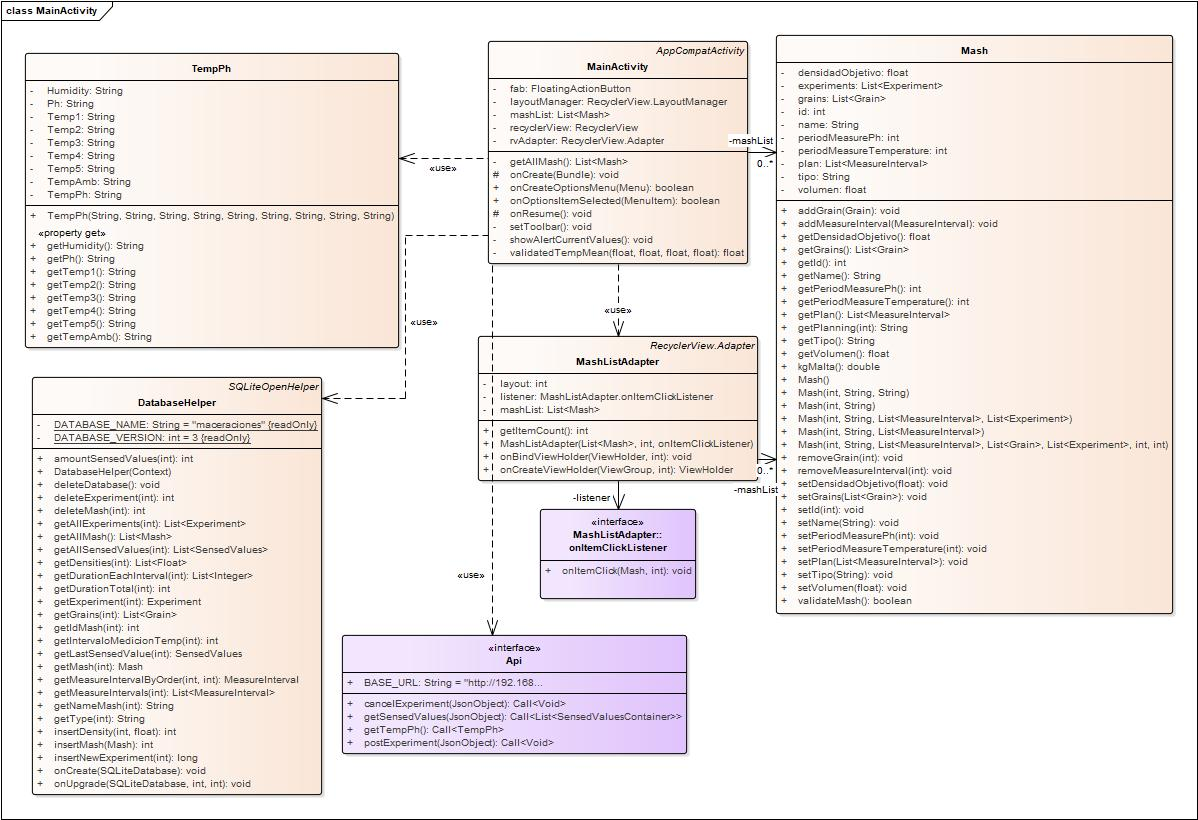
\includegraphics[scale=0.5, angle =90]{Anexo/DiagramasClase/MainActivity.jpg}
        \captionof{figure}{Diagrama de clases de MainActivity}
        \label{fig:DiagClaseMainActivity}
    \end{figure}
    
    
    %\begin{minipage}{0.95\textwidth}
    \begin{figure}
        \centering
        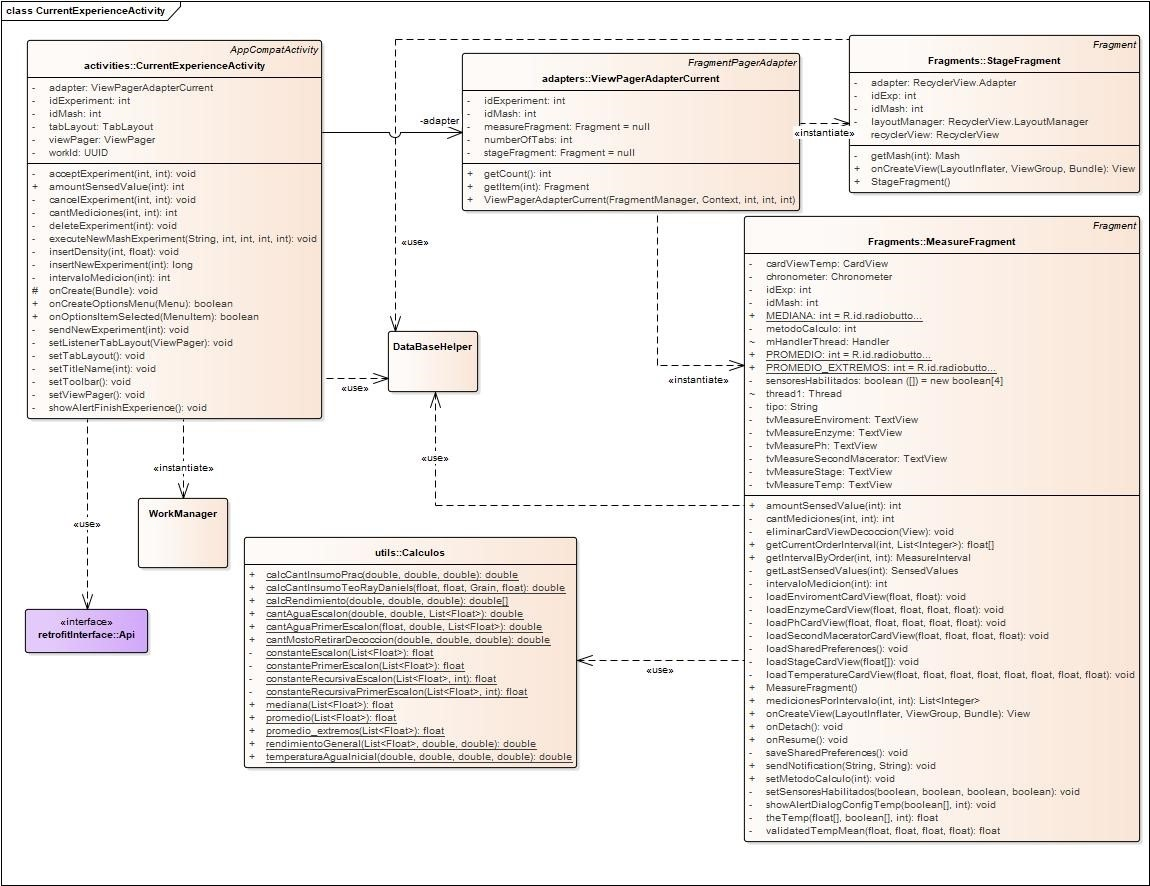
\includegraphics[scale=0.6, angle=90]{Anexo/DiagramasClase/CurrentExperienceActivity-P1.jpg}
        \captionof{figure}{Diagrama de clases de CurrentExperienceActivity - Parte 1}
        \label{fig:DiagClaseCurrentExperienceActivityP1}
    \end{figure}
    %\end{minipage}
    
    %\begin{minipage}{0.95\textwidth}
    \begin{figure}
        \centering
        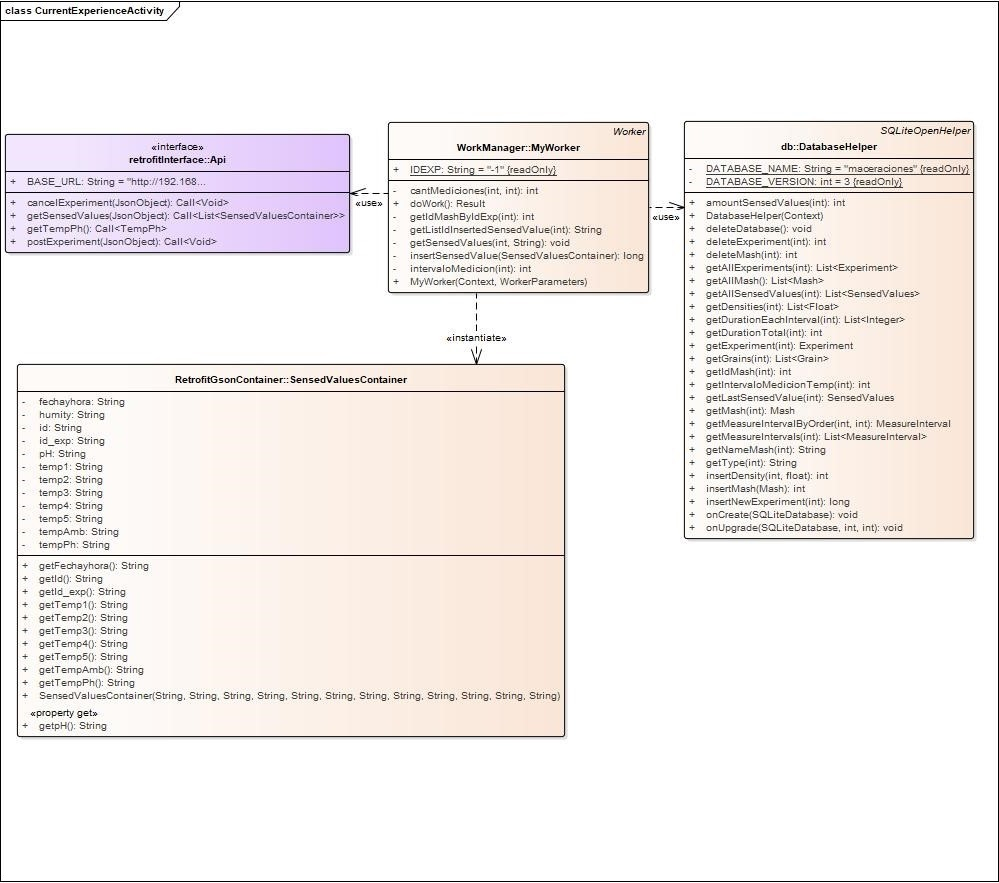
\includegraphics[scale=0.6, angle=90]{Anexo/DiagramasClase/CurrentExperienceActivity-P2.jpg}
        \captionof{figure}{Diagrama de clases de CurrentExperienceActivity - Parte 2}
        \label{fig:DiagClaseCurrentExperienceActivityP2}
    \end{figure}
    %\end{minipage}
    
    %\begin{minipage}{0.95\textwidth}
        \begin{figure}
        \centering
        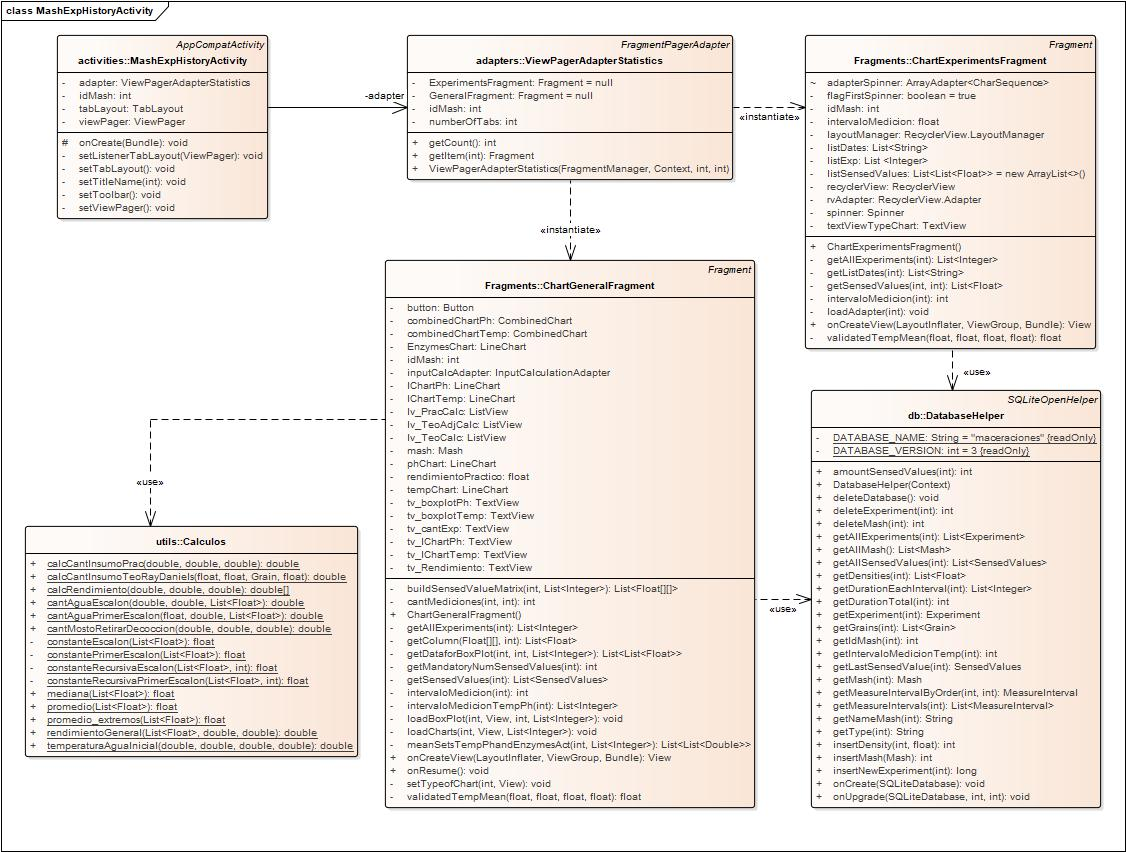
\includegraphics[scale=0.5, angle=90]{Anexo/DiagramasClase/MashExpHistoryActivity.jpg}
        \captionof{figure}{Diagrama de clases de MashExpHistoryActivity}
        \label{fig:DiagClaseMashExpHistoryActivity}
        \end{figure}
    %\end{minipage}
    
    %\begin{minipage}{0.95\textwidth}
        \begin{figure}
        \centering
        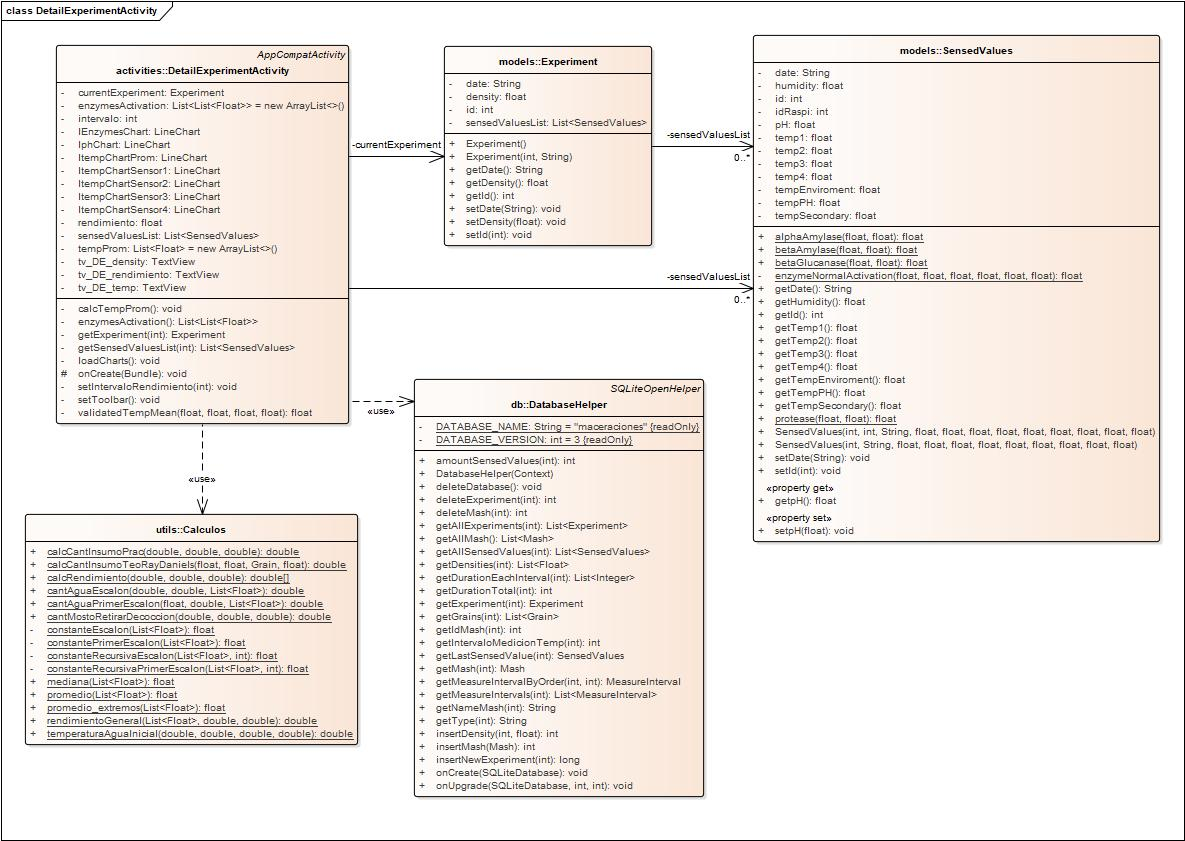
\includegraphics[scale=0.5, angle=90]{Anexo/DiagramasClase/DetailExperimentActivity.jpg}
        \captionof{figure}{Diagrama de clases de DetailExperimentActivity}
        \label{fig:DiagClaseDetailExperimentActivity}
        \end{figure}
    %\end{minipage}
    
    %\begin{minipage}{0.95\textwidth}
        \begin{figure}
        \centering
        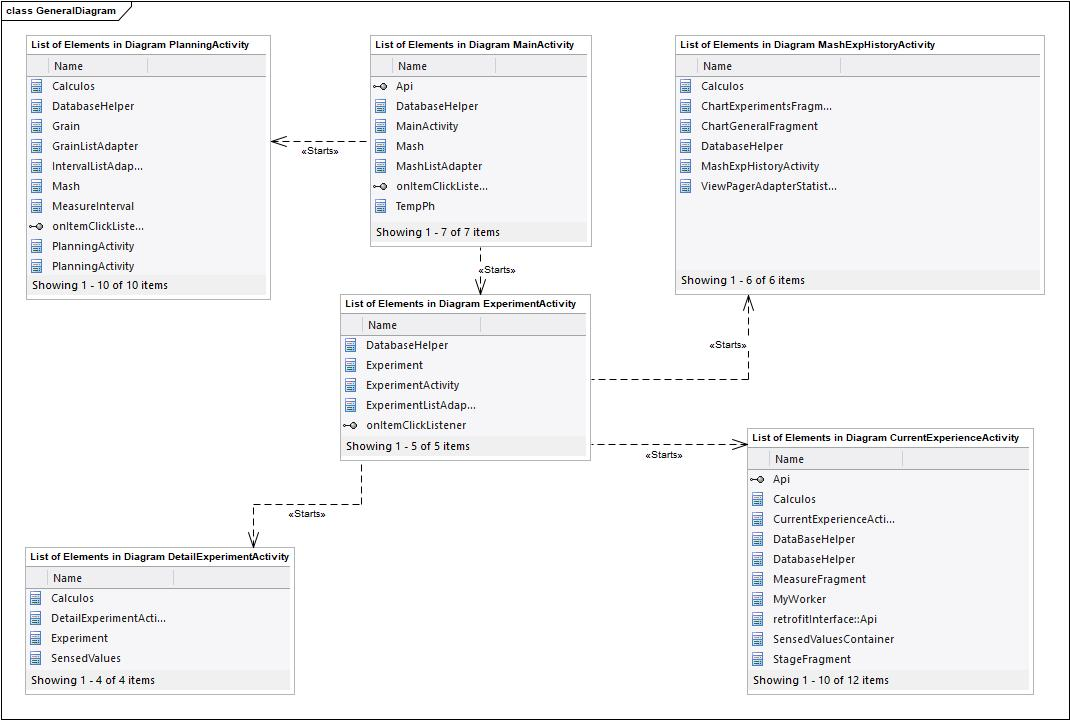
\includegraphics[scale=0.5, angle=90]{Anexo/DiagramasClase/GeneralDiagram.jpg}
        \captionof{figure}{Diagrama General de la APP}
        \label{fig:DiagGeneral}
        \end{figure}
    %\end{minipage}